\usetikzlibrary{shapes,arrows}

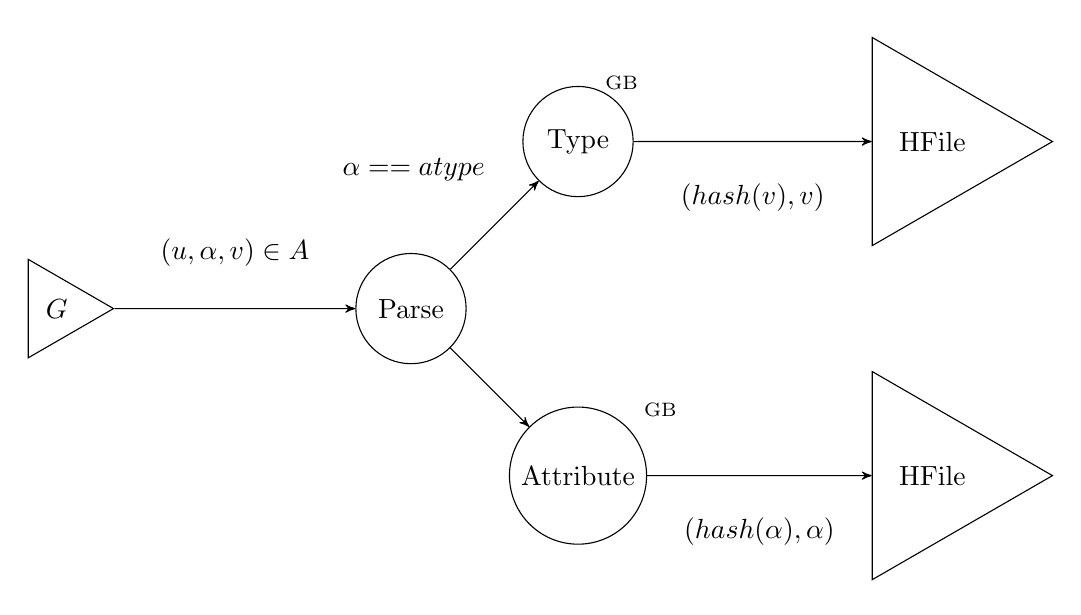
\begin{tikzpicture}[->,>=stealth',node distance=3cm,minimum height=1.4cm]

\node[draw,regular polygon, regular polygon sides=3,shape border rotate=-90] (in) {$G$};

\node[draw,circle,right of = in,xshift=1.5cm] (parse) {Parse};

\node[draw,circle,above right of = parse] (type) {Type};
\node [above right of = parse,label={[label distance=.1cm]10:\scriptsize{GB}}] {};

\node[draw,circle,below right of = parse] (attribute) {Attribute};
\node [below right of = parse,label={[label distance=.6cm]10:\scriptsize{GB}}] {};

\node[right of = type,draw,regular polygon, regular polygon sides=3,shape border rotate=-90,xshift=1.5cm] (tout) {HFile};
\node[right of = attribute,draw,regular polygon, regular polygon sides=3,shape border rotate=-90,xshift=1.5cm] (aout) {HFile};

\path
(in) edge node[above] {$(u, \alpha, v) \in A$} (parse)
(parse) edge node[above left] {$\alpha == \gls{atype}$} (type)
(parse) edge (attribute)
(type) edge node[below] {$(\text{hash}(v), v)$} (tout)
(attribute) edge node[below] {$\left(\text{hash}(\alpha), \alpha\right)$} (aout)
;
\end{tikzpicture}